\scanpage{492}
% 492-01: continuation at the upper edge.
and likewise \deleted{$\unsure{\Psi_{-\mathrm j}^{\pi}}$}
\margin{$\left\{
\begin{gathered}
\Psi_{\unsure{-\overline{\mathrm j}|-\mathrm j}}^{\unsure{\pi}}:
\unsure{\widetilde{\Gamma}'_{\mathbb Q}}\simeq
\unsure{\widetilde{\mathcal T}'_{0,3}}
\longrightarrow T_{\rho}(\widehat{\mathbb Z})/\pm1\\
\unsure{\widetilde{\Gamma}'_{\mathbb Q}}
=\{\gamma\in\widetilde{\Gamma}_{\mathbb Q}\mid
\varepsilon_3(\mu)=1,\ \text{where }\mu=\chi(\gamma)\}
\end{gathered}\right.$}
\margin{\unsure{(50}}

% 492-02: upper paragraph and its left margin.
We thus see that the indeterminacies of the \uline{signs} for
$\Theta_{\rho}^{\unsure{\pi}},\Theta_{\sigma}^{\unsure{\pi}}$
correspond precisely to the indeterminacies for $\Theta_G$
itself --- everything hangs together! The latter is removed
\deleted{\unsure{by} \illegible{2}} tautologically when we replace
$\widetilde M_{0,3}$ by the \deleted{\unsure{covering|profinite} \unsure{with|of} $\unsure{2}$ \unsure{sheets}}
\inserted{ad-hoc extension} $\unsure{\widetilde{\mathcal T}_{1,1}}$ by $\pm1$,
so that we find
\margin{We will \unsure{note} \unsure{however} that $\Theta_{\rho}^{\unsure{\pi}}$,
unlike the splitting $\Psi_{\rho}^{\unsure{\pi}}
=\Psi_{1/2}^{\unsure{\pi}}$, is defined on
$\unsure{\widetilde{\mathcal T}_{0,3}}$ in its entirety.
\figure{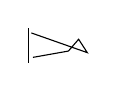
\begin{tikzpicture}
\draw (0,-.22)--(0,.22);
\draw (.04,.16)--(.75,-.09)--(.64,.08)--(.51,-.07)--(.06,-.15);
\end{tikzpicture}}}

% 492-03: display (50).
\[
(50)\qquad \unsure{\widetilde{\mathcal T}_{1,1}}
\longrightarrow \mathrm{GL}(2,\widehat{\mathbb Z})
\]

% 492-04: middle and lower paragraph.
and one should \deleted{\unsure{be able to}} interpret this homomorphism
as the fundamental ``modular'' homomorphism of the theory of elliptic
curves (that the inverse image of \deleted{$\unsure{\Gamma}$}
$\Gamma_{\mathbb Q}\subset\widetilde\Gamma_{\mathbb Q}$ in
$\unsure{\widetilde{\mathcal T}_{1,1}}$ \unsure{can} be interpreted as
$\unsure{\mathcal T_{1,1}}\simeq\pi_1(M_{1,1\,\mathbb Q})$
must be more or less tautological, by construction.)

% 492-05: final paragraph, interlinear addition, and display (51).
It is clear in any case that the two coincide
\inserted{for every $\gamma\in\widetilde M_{0,3}$}
\unsure{viewed} \unsure{as|when} elements of
\[
(51)\qquad \mu_2(\widehat{\mathbb Z})=\{\pm1\}^{\mathbb P}
\qquad (\mathbb P=\text{set of prime numbers})
\]
\mspage{491}

\scanpage{493}
\mspage{549}
% 493-01: continuation, with an overwritten source in the first display.
i.e. they coincide modulo a homomorphism
\[
\deleted{\unsure{M_{0,3}}}\inserted{\unsure{\widetilde\Gamma_{\mathbb Q}}}
\longrightarrow\mu_2(\widehat{\mathbb Z})\simeq\{\pm1\}^{\mathbb P}
\]
i.e. a homomorphism
\[
\begin{aligned}
G_{\mathrm m}(\widehat{\mathbb Z})_2
&=(\widehat{\mathbb Z}^{*})_2\simeq\{\pm1\}^{\mathbb P}
\longrightarrow\deleted{\unsure{\mu}}\unsure{{}_2G_{\mathrm m}}(\widehat{\mathbb Z})
=\mu_2(\widehat{\mathbb Z})\\
&\hspace{24em}\simeq\{\pm1\}^{\mathbb P}
\end{aligned}
\]

% 493-02: middle prose.
--- so it is not a \unsure{certain} indeterminacy that is at issue!
It is morally certain that the two coincide --- I have not tried to
prove it.

% 493-03: lower prose and its interlinear insertion.
As for (35) (36), they must surely correspond to the action of
$\Gamma_{\mathbb Q}$ on the Tate modules of elliptic curves with
exceptional isomorphisms, corresponding precisely to the points
$(1/2,2,-1)$ and $(-\overline{\mathrm j},-\mathrm j)$ of
$M_{0,3\,\mathbb Q}=M_{1,1}[2]'_{\mathbb Q}$.
The indeterminacy of sign \inserted{\unsure{must|of which}} \unsure{correspond|corresponds} to the indeterminacy
in lifting a point of $M_{1,1}[2]'_{\mathbb Q}$ to a point of
$M_{1,1}[2]_{\mathbb Q}$, i.e. in choosing an elliptic curve
(with ``\uline{rigidification}'' of level 2) corresponding to the
\uline{Legendre} data $(0,1,\infty,\unsure{q|\rho})$ with
$\unsure{\rho|q}=1/2$ or $\unsure{\rho|q}=-\overline{\mathrm j}$.
\mspage{492}

\scanpage{494}
% 494-01: upper paragraph.
Even once the \unsure{ambiguity} of sign for
$\Theta_{\unsure{G}}^{\unsure{\pi}}$ is removed by passing to the two-sheeted extension
$\unsure{\widetilde{\mathcal T}_{1,1}}$ of
$\widetilde M_{0,3}$, the indeterminacy of the signs for
$\Theta_{\rho}^{\unsure{\pi}},\Theta_{\sigma}^{\unsure{\pi}}$
is not \unsure{removed} for all that, for the splittings
\deleted{$\unsure{\Psi_{\rho}^{\pi},\Psi_{\sigma}^{\pi}}$}
$\Psi_{1/2}^{\unsure{\pi}},\Psi_{-\overline{\mathrm j}}^{\unsure{\pi}}$)
are not for all that splittings (even partial!)
of \deleted{\unsure{this}} \unsure{the extension}
$\unsure{\widetilde{\mathcal T}_{1,1}}$, but only of
$\widetilde M_{0,3}$ --- and lifting them to splittings of
$\unsure{\widetilde{\mathcal T}_{1,1}}$
\inserted{over $\unsure{\mathcal T_{1,1}}$,}
amounts, very precisely, to choosing precisely elliptic curves with
Legendre rigidification over the points $1/2,-\overline{\mathrm j}$.
Thus, calculations made in terms of automorphisms of the groups with loops
$\widehat\Pi_{0,3}$ \unsure{or} \inserted{of}
$\unsure{\mathcal{C}}_{0,3}^{+\wedge}$,
\unsure{give back} \inserted{(without having \unsure{looked for} them!)}
results that fit very closely with particularly crucial
arithmetico-geometric truths.
\mspage{493}

\scanpage{495}
\mspage{550}
% 495-01: heading.
49.\quad \uline{Homomorphisms of} $M_{0,3}$, the general groups
$M_{\rho,\sigma}$.

% 495-02: left-margin notes.
\margin{\unsure{Where we get our feet wet}\ldots}
\margin{\unsure{All of} this section \inserted{I} \unsure{seems}
entirely useless for what follows, it is a preliminary \unsure{groping}
to lead into section \uline{II} page 553.}

% 495-03: first paragraph.
I) Consider a \inserted{closed} subgroup $G$ of $M_{0,3}$,
containing $\unsure{\mathcal C}_{0,3}^{+\wedge}$, hence the inverse image of a
closed subgroup of $\widetilde\Gamma_{0,3}$.
We assume that the latter is ``big enough'' --- say that it contains
a subgroup of finite index in
$\Gamma_{\mathbb Q}\subset\widetilde\Gamma_{0,3}$.
For the moment, we assume for simplicity that $G\subset\operatorname{Ker}\varepsilon_3$.
In summary
\[
(1)\qquad
\unsure{\mathcal C}_{0,3}^{+\wedge}\subset G\subset\widetilde M_{0,3},
\qquad u\in G\Longrightarrow\mu(u)\equiv1\ (3).
\]

% 495-04: interlinear correction and parallel maps.
This last hypothesis thus \deleted{implies}\inserted{means} that
for every $u\in G$, we have $\alpha_0(u)\in\unsure{\mathcal C}_{0,3}^{\wedge+}$,
so we have
\[
(\unsure{2})\qquad
\diagram{\begin{tikzcd}[column sep=large]
G \arrow[r,shift left=.7ex,"\underline{\alpha}_0"]
  \arrow[r,shift right=.7ex,"\underline{\beta}_0"']
& \unsure{\mathcal C}_{0,3}^{+}
\end{tikzcd}},
\]
characterized by
\[
(2')\qquad
\left\{\begin{aligned}
u(\rho)&=\operatorname{int}(\alpha_0)\rho\\
u(\sigma)&=\operatorname{int}(\beta_0)\sigma
\end{aligned}\right.
\qquad
\begin{aligned}
\alpha_0&=\underline{\alpha}_0(u)\\
\beta_0&=\underline{\beta}_0(u).
\end{aligned}
\]

% 495-05: the vertically arranged subgroups, including the intervening sign.
We consider
\[
(3)\qquad
\begin{array}{l}
G(0)=G\cap\widetilde M_{0,3}(0)\\[-.4em]
\quad\cap\\[-.4em]
G[0]=G\cap\widetilde M_{0,3}[0]=\operatorname{Norm}_{G}(L_0^{\unsure{\mathcal C}})
\end{array}
\]
so that
\[
\begin{aligned}
(4)\qquad&G=G(0).\unsure{\mathcal C}_{0,3}^{+\wedge}
&&\text{(semidirect product)}\\
(5)\qquad&G[0]=G(0).L_0^{\unsure{\mathcal C}}
&&\text{id}\\
(6)\qquad&G[0]\cap\unsure{\mathcal C}_{0,3}^{+\wedge}
=L_0^{\unsure{\mathcal C}}.
\end{aligned}
\]

% 495-06: definition (7) and last line.
We have set
\[
(7)\qquad
\begin{gathered}
L_0^{\unsure{\mathcal C}}=\text{closed subgroup of }
\unsure{\mathcal C}_{0,3}^{+\wedge}\text{ generated}\\
\text{by }\varepsilon_0
\end{gathered}
\]
and we define likewise $L_1^{\unsure{\mathcal C}},L_{\infty}^{\unsure{\mathcal C}}$.
\mspage{494}

\scanpage{496}
% 496-01: paragraph and first map, with changes of target notation.
Consider a \inserted{profinite} group
$\deleted{\unsure{A}}\inserted{M}$, and a \inserted{(continuous)}
\uline{surjective} homomorphism
\[
(8)\qquad \varphi:G\longrightarrow\deleted{\unsure{A}}M.
\]
We set
\[
(9)\quad
\left\{\begin{aligned}
\varphi(\unsure{\mathcal C}_{0,3}^{+\wedge})
 &=\unsure{\mathcal C}\qquad\text{normal subgroup of }M\\
\varphi(G(0))&=\deleted{\unsure{A}}\inserted{M}(0)\\
\varphi(G[0])&=\deleted{\unsure{A}}\inserted{M}[0].\\
\varphi(L_0^{\unsure{\mathcal C}})&=L_0^{\deleted{\unsure{\mathcal C}}}
\end{aligned}\right.
\]

% 496-02: subgroup relations.
\deleted{\unsure{Thus}}

Thus these are closed subgroups of $M$, satisfying
\[
\begin{aligned}
(10)\qquad&M(0)\subset M[0]\subset\operatorname{Norm}_{M}(L_0)\\
(11)\qquad&L_0^{\deleted{\unsure{\mathcal C}}}
\subset\unsure{\mathcal C}\cap M[0].
\end{aligned}
\]

% 496-03: the surviving generator relations.
By abuse of language, we still denote by $\rho,\sigma,\varepsilon_0,\varepsilon_1$
\ldots\ the images of these elements in $\unsure{\mathcal C}$, which
therefore satisfy there the relations known in $\unsure{\mathcal C}_{0,3}^{+\wedge}$,
in particular
\[
(12)\qquad
\sigma^2=\rho^3=1,\qquad
\sigma\rho=\varepsilon_0,\quad \rho\sigma=\varepsilon_1,\qquad
\varepsilon_1=\sigma(\varepsilon_0)=\rho(\varepsilon_0).
\]

% 496-04: paragraph and revised definition (13).
The restrictions of the maps $\alpha_0,\beta_0$ of (2,2') to
$M_{\rho,\sigma}[0]$ will rather be denoted $\alpha,\beta$, where $\alpha,\beta$
are in fact maps
\[
(13)\quad
\diagram{\begin{tikzcd}[column sep=large]
{\begin{gathered}
SG\overset{\mathrm{dfn}}=\deleted{\text{extension of}}\ G\\
\text{by }L_0^{\unsure{\mathcal C}},\ \text{inverse}\\
\text{image of }\unsure{G}\\
\text{in }S\widetilde M_{0,3}\\
=\{(u,f)\in G\times\unsure{\mathcal C}_{0,3}^{+\wedge}\mid fu\in G[0]
\end{gathered}}
\arrow[r,shift left=.7ex,"\alpha"]
\arrow[r,shift right=.7ex,"\beta"']
&\unsure{\mathcal C}_{0,3}^{+\wedge}
\end{tikzcd}}
\]
of which we look at the restrictions to the \uline{subgroup}
($\simeq M_{\rho,\sigma}[0]$) of $SG$ defined by the relation $f=1$.

% 496-05: composition of the two functions, and (14).
Composing $\underline\alpha,\underline\beta:$
\diagram{\begin{tikzcd}[column sep=small]
\deleted{\unsure{M[0]}}\inserted{G[0]}
\arrow[r,shift left=.5ex]\arrow[r,shift right=.5ex]
&\unsure{\mathcal C}_{0,3}^{+\wedge}
\end{tikzcd}}
with $\varphi\mid\unsure{\mathcal C}_{0,3}^{+\wedge}$, we find
maps, again denoted $\underline\alpha,\underline\beta$
(where $\underline\alpha^M,\underline\beta^M$ in case of possible confusion)
\[
(14)\qquad
\diagram{\begin{tikzcd}[column sep=large]
G[0]\arrow[r,shift left=.7ex,"\underline\alpha"]
\arrow[r,shift right=.7ex,"\underline\beta"']
&\unsure{\mathcal C}
\end{tikzcd}}
\]
thus satisfying
\[
(15)\qquad
\left\{\begin{aligned}
\unsure{u}(\rho)&=\operatorname{int}(\alpha)\rho\\
\unsure{u}(\sigma)&=\operatorname{int}(\beta)\sigma
\end{aligned}\right.
\qquad
\begin{gathered}
\text{for }u\in M[0]\ \inserted{\text{\unsure{of}}}\text{ the form }\varphi(u_0),\\
\text{and }\alpha=\underline\alpha(u_0),\ \beta=\underline\beta(u_0).
\end{gathered}
\]
\mspage{495}

\scanpage{497}
\mspage{551}

% 497-01
A priori, $\alpha$ and $\beta$ depend on the choice of $u_0$ from which $u$ comes
not only on $u$ --- but
% 497-02
\[
(16)\qquad
\left\{\begin{aligned}
\alpha\rho(\alpha)^{-1}&=[u,\rho]\\
\beta\sigma(\beta)^{-1}&=[u,\sigma]
\end{aligned}\right.
\]
% 497-03
do not depend on it. If we put
% 497-04
\[
(17)\qquad
T_{\rho}=\uline{\mathrm{Centr}}_M(\rho)
\qquad
T_{\sigma}=\uline{\mathrm{Centr}}_M(\sigma)
\]
% 497-05
we thus see that, modulo $T_{\rho}$ resp. $T_{\sigma}$,
$\alpha,\beta$ depend only on $u$.

% 497-06, 497-07, 497-08, 497-09
\uline{Hypothesis}
$\alpha\inserted{{}=\alpha(u_0)},\beta\inserted{{}=\beta(u_0)}$
depend only on $u=\varphi(u_0)$
(for $u_0\in\deleted{\unsure{M}}\unsure{G}[0]$).

% 497-10
We shall \unsure{express} this hypothesis in a slightly different way,
by introducing
% 497-11
\[
(18)\qquad J=\operatorname{Ker}(G[0]\longrightarrow M[0]),
\]
% 497-12, 497-13
we thus want that for $\deleted{\unsure{\alpha}}$
% 497-14, 497-15
\[
u'_0=\deleted{u_0}\delta_0u_0\quad
\text{with }u_0\in G[0],\ \delta_0\in J,\quad\text{we have}
\]
% 497-16
\[
\alpha(u'_0)=\alpha(u_0),\qquad \beta(u'_0)=\beta(u_0)
\]
% 497-17, 497-18
\unsure{Write}
\[
\begin{gathered}
\alpha_0=\uline{\alpha}(u_0),\quad
\beta_0=\uline{\beta}(u_0),\quad
\alpha'_0=\uline{\alpha}(u'_0),\quad
\beta'_0=\uline{\beta}(u'_0),\quad
\overline{\alpha}_0=\uline{\alpha}(\delta_0),\quad
\overline{\beta}_0=\uline{\beta}(\unsure{\delta_1|\delta_0}),
\end{gathered}
\]
\uline{in} $G$, so that we shall have, by the cocycle formulas of $G$
% 497-19
\[
\alpha'_0=\delta_0(\alpha_0)\overline{\alpha}_0,
\qquad
\beta'_0=\delta_0(\beta_0)\overline{\beta}_0,
\]
% 497-20
whence, applying $\varphi$ and noting that
% 497-21
\[
\begin{aligned}
\varphi(\delta_0(\alpha_0))
&=\underbrace{\varphi(\delta_0)}_{1}(\varphi(\alpha_0))
=\varphi(\alpha_0)\overset{\mathrm{dfn}}=\alpha
&&\text{and likewise}\\
\varphi(\delta_0(\beta_0))&=\varphi(\beta_0)\overset{\mathrm{dfn}}=\beta
\end{aligned}
\]
% 497-22, 497-23
\[
(19)\qquad
\alpha'=\deleted{\unsure{\varphi}}\alpha\overline{\alpha},\qquad
\beta'=\beta\overline{\beta}\qquad\text{in }\unsure{\mathcal{C}}
\]
% 497-24, 497-25
where $\alpha,\beta,\alpha',\beta',\overline{\alpha},\overline{\beta}$ are the images under
$\varphi$ of the quantities $\alpha_0$ etc in $\unsure{\mathcal{C}}_{0,3}^{+\wedge}$.
\deleted{\unsure{with} $\alpha=\alpha(u_0)$}
Thus the hypothesis means this
% 497-26
\[
(20)\qquad
\forall\,\delta_0\in J\overset{\mathrm{dfn}}=
\operatorname{Ker}(G[0]\longrightarrow M[0]),\quad
\text{we have}\quad
\unsure{\alpha^{\Pi}}(\delta_0),\unsure{\beta^{\Pi}}(\delta_0)
\in\unsure{\operatorname{Ker}}\varphi
\]
% 497-27, 497-28
\deleted{\unsure{when}}
When this hypothesis is satisfied, we thus have maps
\mspage{496}

\scanpage{498}

% 498-01
\[
(21)\qquad
\diagram{\begin{tikzcd}[column sep=large]
M[0]\arrow[r,shift left=0.65ex,"\uline{\alpha}"]
\arrow[r,shift right=0.65ex,"\uline{\beta}"']&\unsure{\mathcal{C}}
\end{tikzcd}}
\]
% 498-02, 498-03
\deleted{satisfying}
\unsure{factoring} (14), and thus satisfying
% 498-04
\[
(22)\qquad
\left\{\begin{aligned}
u(\rho)&=\operatorname{int}(\alpha)\rho\\
\unsure{u}(\sigma)&=\operatorname{int}(\beta)\sigma
\end{aligned}\right.
\qquad
\text{for }\unsure{u}\in M[0],\quad
\alpha=\uline{\alpha}(u),\quad\beta=\uline{\beta}(u),
\]
% 498-05, 498-06, 498-07
which \deleted{\unsure{generalize|generalizing}}
\inserted{\unsure{paraphrase}} (2').

% 498-08
Moreover, let us put
% 498-09
\[
(23)\qquad
\unsure{\zeta|\xi}=\alpha\rho(\alpha)^{-1},\qquad
\eta=\beta\sigma(\beta)^{-1}
\]
% 498-10
the relations (22) can be written thus
% 498-11
\[
(24)\qquad u(\rho)=\unsure{\zeta|\xi}\rho,\qquad u(\sigma)=\eta\sigma
\]
% 498-12
and we shall have
% 498-13
\[
(25)\qquad \unsure{\zeta|\xi}=[u,\rho],\qquad \eta=[u,\sigma]
\]
% 498-14
and moreover
% 498-15
\[
(26)\qquad
\unsure{\zeta|\xi}=\eta\unsure{\varepsilon_1|\ell_1}^{\nu}\qquad
\text{where }\nu=\frac{\mu-1}{2}\in\widehat{\mathbb Z}
\quad\text{($\mu$ the multiplier of $u$).}
\]
% 498-16
which comes from the single relation in $\unsure{\mathcal{C}}_{0,3}^{+}$.

% 498-17
(We assume to fix ideas that the homomorphism
% 498-18, 498-19
\[
\deleted{\unsure{(27)}}\qquad
\diagram{\begin{tikzcd}[column sep=large]
G\arrow[r,"\chi^{G}"]&\widehat{\mathbb Z}^{*}
\end{tikzcd}}
\qquad\text{(``multiplier'')}
\]
% 498-20
factors through
% 498-21
\[
(27)\qquad
\diagram{\begin{tikzcd}[column sep=large]
G\arrow[r]&M\arrow[r,"\chi^{M}"]&\widehat{\mathbb Z}^{*},
\end{tikzcd}}
\]
% 498-22
so that we have a notion of multiplier ($\in\widehat{\mathbb Z}^{*}$)
for the $u\in M$.)

% 498-23
Consider the natural homomorphism
% 498-24
\[
(28)\qquad
\diagram{\begin{tikzcd}[column sep=large,row sep=small]
M[0]\arrow[r]&\operatorname{Aut}(\unsure{\mathcal{C}}):\\
u\arrow[r,mapsto]&\operatorname{int}(u)|\unsure{\mathcal{C}}
\end{tikzcd}}
\]
% 498-25, 498-26
we see from (22) \inserted{\unsure{even|or even} (24)}
that it is known when we know
\mspage{497}

\scanpage{499}
\mspage{552}

% 499-01, 499-02
\margin{for \deleted{\illegible{1}} $\rho,\sigma$ generate
\unsure{topologically} $\unsure{\mathcal{C}}$}
% 499-03
the functions $\uline{\alpha},\uline{\beta}:M[0]\longrightarrow\unsure{\mathcal{C}}$,
and even when we know only
$\unsure{\zeta|\xi},\eta:M[0]\longrightarrow\unsure{\mathcal{C}}$.
If moreover we put
% 499-04
\[
(29)\qquad
M'[0]=\operatorname{Im}(M[0]\longrightarrow\operatorname{Aut}(\unsure{\mathcal{C}}))
\]
% 499-05
these latter functions $\unsure{\zeta|\xi},\eta$ are already defined on $M'[0]$ --- whereas it
is not clear that the same holds for $\alpha,\beta$, when
$M[0]$ \unsure{does not act|does not operate} faithfully on $\unsure{\mathcal{C}}$.
We thus have a map \inserted{$(\unsure{\zeta|\xi},\eta)$} from a certain subgroup
$M'[0]\subset\operatorname{Norm}_{\operatorname{Aut}(\unsure{\mathcal{C}})}(L_0)$
to the set $\unsure{\mathcal{R}}$ of solutions of the equation in $\unsure{\zeta|\xi},\eta$
(26) which we \unsure{write|shall write} simply
% 499-06
\[
(30)\qquad \eta^{-1}\unsure{\zeta|\xi}\in L_1
\]
% 499-07, 499-08
a relation which implies (26) (with the precise form of the exponent $\nu$)
if we assume \inserted{(\unsure{for example})} $\unsure{\mathcal{C}|M}$ big enough that
% 499-09
\inserted{$\diagram{\begin{tikzcd}[column sep=large]
\unsure{\mathcal{C}}_{0,3}^{+\wedge}\arrow[r,"\unsure{2}"']&
\unsure{\mathrm{SL}|\mathrm{PSL}}(2,\widehat{\mathbb Z})
\end{tikzcd}}$}
factors through $\unsure{\mathcal{C}}$ --- which we shall assume, to make life easier for ourselves.

% 499-10, 499-11
\deleted{We shall make on $\unsure{\mathcal{C}}$, equipped with $\rho,\sigma,\varepsilon_1$
the following hypothesis}
\inserted{More precisely, let}
% 499-12
\deleted{(31) \unsure{H)|II)} On}
% 499-13, 499-14, 499-15, 499-16
\[
(32)\qquad
\left\{\begin{gathered}
\deleted{\unsure{\Sigma|\mathcal{R}}}\ \unsure{=}
\Sigma_{\unsure{\mathcal{C}},\rho,\sigma}
\subset\unsure{\mathcal{C}}\times\unsure{\mathcal{C}}\\
\Vert\\[-1ex]
\left\{(\unsure{\zeta|\xi},\eta)\ \middle|
\begin{array}{ll}
\text{a)}&\unsure{\zeta|\xi}\rho\ \text{conjugate to }\rho\quad
\deleted{\text{in }\operatorname{Aut}(\unsure{\mathcal{C}})}
\inserted{\text{in }\unsure{\mathcal{C}}}\\[1ex]
\text{b)}&\eta\sigma\quad\rule{2.7cm}{0.4pt}\quad\sigma\quad\rule{2cm}{0.4pt}\\[1ex]
\text{c)}&\eta^{-1}\unsure{\zeta|\xi}\in L_1\quad\text{i.e.}\quad
\exists\nu'\in\widehat{\mathbb Z}\ \text{such that }\unsure{\zeta|\xi}=\eta\varepsilon_1^{\nu'}
\end{array}\right\}
\end{gathered}\right.
\]
% 499-17, 499-18
\margin{\[
\begin{gathered}
\underbrace{[\alpha,\rho]=\alpha\rho(\alpha)^{-1}}\\
\left\{\begin{array}{l}
\text{\unsure{i.e.} }\unsure{\zeta|\xi}\ \text{\unsure{of the form} }\unsure{[\alpha,\rho]}\\
\text{\unsure{resp.} }\eta\ \text{\unsure{of the form} }\unsure{[\beta,\sigma]}
\unsure{{}=\beta\sigma(\beta)^{-1}}
\end{array}\right.
\end{gathered}
\]}

% 499-19, 499-20, 499-21, 499-22, 499-23
\deleted{For \unsure{every} $u\in\operatorname{Aut}(\unsure{\mathcal{C}})$
\uline{normalizing} $L_0$, \deleted{and \unsure{fixing}}
\deleted{\unsure{must}} and fixing the conjugacy class of
$\rho$ and that of $\sigma$, i.e. \unsure{such|such} that
\[
\deleted{\unsure{\zeta|\xi}=[u,\rho]}\qquad(\unsure{\zeta|\xi},\eta)=([u,\rho],[u,\sigma])
\]
\unsure{satisfy|satisfies} the first two conditions of (33), \unsure{and}}
\mspage{498}

\scanpage{500}

% 500-01
and let $u\in\operatorname{Aut}(\unsure{\mathcal{C}})$ be an automorphism of
$\unsure{\mathcal{C}}$, and let us put
% 500-02
\[
(34)\qquad
\left\{\begin{aligned}
\unsure{\zeta|\xi}&=[u,\rho]=u\rho u^{-1}\rho^{-1}=u(\rho)\rho^{-1}
&&\text{i.e. }u(\rho)=\unsure{\zeta|\xi}\rho\\
\eta&=[u,\sigma]=u(\sigma)\sigma^{-1}
&&\text{i.e. }u(\sigma)=\eta\sigma
\end{aligned}\right.
\]
% 500-03
\margin{cf. (24),(25)}
% 500-04, 500-05, 500-06
then to say that $\unsure{\zeta|\xi}\rho$ \inserted{$(=u(\rho))$} is conjugate to $\rho$ means
that $u$ fixes the conjugacy class of $\rho$, to say that $\eta\sigma$
\inserted{$(=u(\sigma))$} is conjugate \unsure{of|to} $\sigma$ means that $u$ fixes
the conjugacy class of $\sigma$.
Finally the condition $\eta^{-1}\unsure{\zeta|\xi}\in L_1$ can also be written, since
% 500-07, 500-08
\[
\begin{aligned}
\eta^{-1}\unsure{\zeta|\xi}
&=(\sigma u(\sigma^{-1}))(u(\rho)\rho^{-1})
=\sigma u(\sigma^{-1}\rho)\rho^{-1}\\
&=\sigma\left(u(\underbrace{\sigma^{-1}\rho}_{\varepsilon_0})
\deleted{\unsure{\sigma}}\underbrace{\rho^{-1}\sigma}_{\varepsilon_0^{-1}}\right)
\end{aligned}
\]
% 500-09
\margin{N.B. $\sigma^{-1}=\sigma$}
% 500-10, 500-11
\deleted{\unsure{whence}}
\[
{}=\sigma(u(\varepsilon_0)\varepsilon_0^{-1})
\]
% 500-12
in the form
% 500-13
\[
\sigma(u(\varepsilon_0)\varepsilon_0^{\unsure{-1}})\in L_1
\qquad\text{i.e.}\qquad
u(\varepsilon_0)\varepsilon_0^{-1}\in L_0
\]
% 500-14, 500-15, 500-16
(since $L_0=\sigma^{-1}(L_1)$) or again
(since $\varepsilon_0$ \deleted{generates}\inserted{$\in L_0$})
% 500-17
\[
u(\varepsilon_0)\in L_0,\quad
\text{i.e. (since $\varepsilon_0$ generates $L_0$)}
\]
% 500-18
\margin{In this argument, we have used only the relation
$\sigma^{-1}\rho=\varepsilon_0$ and the fact that $\varepsilon_0$ generates $L_0$,
\unsure{and not} that $\sigma^2=1$ or $\rho^3=1$ for example.}
% 500-19
\[
u(L_0)=L_0
\]
% 500-20
i.e. that $u$ \uline{normalizes} $L_0$.

% 500-21
Thus let
% 500-22
\[
(35)\qquad
\left\{\begin{gathered}
\widetilde{B}'_0\subset\operatorname{Aut}(\unsure{\mathcal{C}})\\
\Vert\ \mathrm{dfn}\\[-1ex]
\left\{u\in\operatorname{Aut}(\unsure{\mathcal{C}})\ \middle|
\begin{array}{l}
u\ \text{fixes conjugacy \unsure{class} of $\rho$ and that of $\sigma$}\\
u\ \text{normalizes }L_0
\end{array}\right\},
\end{gathered}\right.
\]
% 500-23
so that we have a map (injective because $\rho,\sigma$ generate
$\unsure{\mathcal{C}}$)
% 500-24
\[
(36)\qquad
\diagram{\begin{tikzcd}[column sep=large,row sep=small]
\widetilde{B}'_0\arrow[r,hook]&\Sigma\\
u\arrow[r,mapsto]&([u,\rho]=u(\rho)\rho^{-1},\ [u,\sigma]=u(\sigma)\sigma^{-1}).
\end{tikzcd}}
\]
\mspage{499}

\scanpage{501}
\mspage{553}

% 501-01--07: heading, double marginal rule, hypothesis and its alterations.
\[
(37)\quad
\begin{array}{||l}
\text{\uline{Fundamental hypothesis on} }\unsure{\mathcal{C}},\ 
\text{\uline{equipped with} }\rho,\sigma,\ 
\text{\deleted{and}\inserted{\uline{whence}} }\varepsilon_0=\sigma^{-1}\rho,\\[1ex]
\varepsilon_1=\rho\sigma^{-1}=\sigma(\varepsilon_0)=\rho(\varepsilon_0):\\[1ex]
\text{a) }\unsure{\mathcal{C}}\text{ is generated topologically by }\rho,\sigma\\[1ex]
\text{b) The map (36) \deleted{\unsure{is|by}} (injective by a)) is}\\
\text{\phantom{b) }bijective.}
\end{array}
\]

% 501-08--10: canceled first version and its replacement.
\deleted{This thus means that $\forall(\unsure{\zeta|\xi},\eta)\in\Sigma$ \unsure{is|u}}

Condition b) thus means that for
\deleted{of the form $u$,}
$(\alpha,\beta)\in\unsure{\mathcal{C}}\times\unsure{\mathcal{C}}$,
satisfying a relation
\[
\uline{\alpha\rho(\alpha)^{-1}}
=\uline{\beta\sigma(\beta)^{-1}}\varepsilon_1^{\nu'},
\qquad \unsure{\nu''|\nu'}\text{ suitable},
\]
there exists $u\in\operatorname{Aut}(\unsure{\mathcal{C}})$ such that we have
% 501-12--14: two identities, including the canceled right-hand attempt.
\[
\begin{array}{lll}
[u,\rho]=\alpha\rho(\alpha)^{-1}&
\text{i.e. }u(\rho)=\operatorname{int}(\alpha)(\rho)&
\text{i.e. }\inserted{\unsure{u(\rho)|u\rho)}=\unsure{\zeta|\xi}\rho}
\deleted{\unsure{\operatorname{int}(\unsure{\zeta|\xi})\rho}}\\[1ex]
[u,\sigma]=\beta\sigma(\beta)^{-1}&
\text{i.e. }u(\sigma)=\operatorname{int}(\beta)\sigma&
\text{i.e. }u(\sigma)=\eta\sigma
\end{array}
\]

% 501-15: prose continuation (tilde is not visible on this B).
\margin{$\unsure{\bullet}$}
(we shall thus necessarily have $u\in B'_0\ \unsure{\}}$, and
$u$ will be unique if \unsure{we have} a)).

% 501-16--18: final paragraph and overwritten subscript.
Thus, on the set \unsure{of the|of} $\unsure{R|\mathcal{R}}_{\rho,\sigma}$ of the $(\unsure{\zeta|\xi},\eta)$ satisfying
a) b) c), we shall have a group structure, \unsure{+|and} \unsure{deduced|described} by transport of structure from that of
$\widetilde{B}'_{\deleted{\unsure{\rho}}0}$

\unsure{etc.}

\mspage{500}

\scanpage{502}
\margin{\uline{The groups} $M_{\rho,\sigma}$ \uline{etc}}

II Let us return to the situation above, forgetting (at least for the moment) $G$, $\varphi$ etc.

\margin{For a \unsure{systematic} rectification of the notations \unsure{that follow|following} cf. page 564, \uline{remark}.}

Let $\unsure{\mathcal{C}}$ be a group --- we place ourselves, for what follows, either in the category of discrete groups, or in that of profinite groups, as we choose. We shall (to fix ideas) take that of profinite groups. We suppose given
\[
(1)\qquad \rho,\sigma\in\unsure{\mathcal{C}}
\]
\margin{[\unsure{i.e. we have between} $\varepsilon_0=\ell'_0$, $\sigma=\ell'_1$ and $\rho^{-1}=\ell'_\infty$ with relation (2) $\ell'_\infty\ell'_1\ell'_0=1$]}
we put
\[
\varepsilon_0=\sigma^{-1}\rho,\qquad
\varepsilon_1=\rho\sigma^{-1}=\sigma(\varepsilon_0)=\rho(\varepsilon_0)
\]
\[
(3)\qquad
\begin{aligned}
L_0&=\text{closed subgroup generated by }\varepsilon_0\\
L_1&=\rule{6.5cm}{0.3pt}\quad\varepsilon_1
\end{aligned}
\qquad\unsure{\text{, i.}}
\]
thus $L_1=\rho(L_0)=\sigma(L_0)$.

We \deleted{suppose} consider
\diagram{\begin{tikzcd}
\mathrm{Aut}(\unsure{\mathcal{C}}) \arrow[r,"\Phi=(\underline{\unsure{\zeta|\xi}},\underline{\eta})","\deleted{\unsure{\varphi}}"'] & \deleted{\unsure{\mathcal{C}}}\,\unsure{\mathcal{C}}\times\unsure{\mathcal{C}}
\end{tikzcd}}\hfill(4)
defined by
\[
(5)\quad
\left\{\begin{aligned}
\underline{\unsure{\zeta|\xi}}(u)&=[u,\rho]=u\rho u^{-1}\rho^{-1}=u(\rho)\rho^{-1}
&&\text{thus }u(\rho)=\unsure{\zeta|\xi}\rho\quad(\unsure{\zeta|\xi}=\underline{\unsure{\zeta|\xi}}(u))\\
&=u\rho(u)^{-1}\\
\underline{\eta}(u)&=[u,\sigma]=u\sigma u^{-1}\sigma^{-1}=u(\sigma)\sigma^{-1}
&&\text{thus }u(\sigma)=\eta\sigma\quad(\eta=\underline{\eta}(u))\\
&=u\sigma(u)^{-1}.
\end{aligned}\right.
\]
Thus for $u\in\mathrm{Aut}(\unsure{\mathcal{C}})$, and $\unsure{\zeta|\xi}=\underline{\unsure{\zeta|\xi}}(u)$, $\eta=\underline{\eta}(u)$, we have
\[
\unsure{(6)|(5)}\quad
\left\{\begin{aligned}
&u\text{ fixes the }\inserted{\unsure{\mathcal{C}}}\text{-conjugation class of }\rho
\quad\Longleftrightarrow\quad \unsure{\zeta|\xi}\rho\text{ conjugate to }\rho\\
&\hspace{6cm}\Longleftrightarrow\quad\unsure{\zeta|\xi}=\alpha\rho(\alpha)^{-1}\quad(\alpha\in\unsure{\mathcal{C}})\\
&u\text{ fixes the }\unsure{\mathcal{C}}\text{-conjugation class of }\sigma
\quad\Longleftrightarrow\quad \eta\sigma\text{ conjugate to }\sigma\\
&\hspace{6cm}\Longleftrightarrow\quad\eta=\beta\sigma(\beta)^{-1}\quad(\beta\in\unsure{\mathcal{C}})\\
&u\text{ normalizes }L_0\quad\Longleftrightarrow\quad\eta^{-1}\unsure{\zeta|\xi}\in L_1
\quad\Longleftrightarrow\quad\unsure{\zeta|\xi}=\eta\varepsilon_1^\nu\quad\text{with }\nu\in\widehat{\mathbb Z}\text{ suitable}.
\end{aligned}\right.
\]
\mspage{501}

\scanpage{503}
\mspage{554}
\unsure{Let|Let} \deleted{$\unsure{B_{\rho,\sigma}}\subset$}
\[
(7)\qquad
\begin{aligned}
B_{\rho,\sigma}&\subset\mathrm{Aut}(\unsure{\mathcal{C}})\\[-2pt]
\Vert\quad&\\[-10pt]
\{u\mid{}&\text{satisfying the three conditions }(\unsure{6|5})\}
\end{aligned}
\]
\[
(8)\qquad
\begin{gathered}
\Sigma_{\rho,\sigma}\subset\unsure{\mathcal{C}}\times\unsure{\mathcal{C}}\\[-2pt]
\Vert\\[-2pt]
\left\{(\unsure{\zeta|\xi},\eta)\ \middle|\ 
\begin{aligned}
\unsure{\zeta|\xi}&=\alpha\rho(\alpha)^{-1},\quad
\eta=\beta\sigma(\beta)^{-1}\quad(\alpha,\beta\in\unsure{\mathcal{C}})\\
&\inserted{\text{i.e. }\unsure{\zeta|\xi}\rho\text{ conjugate to }\rho,\qquad\text{i.e. }\eta\sigma\text{ conjugate to }\sigma}\\
\eta^{-1}\unsure{\zeta|\xi}&\in L_1\quad\text{i.e. }\unsure{\zeta|\xi}=\eta\varepsilon_1^\nu\quad(\nu\in\widehat{\mathbb Z})
\end{aligned}\right\},
\end{gathered}
\]
so that $B_{\rho,\sigma}$ is the inverse image of $\Sigma_{\rho,\sigma}$ under (4), and we have an induced map
\diagram{\begin{tikzcd}
B_{\rho,\sigma}\arrow[r,"\varphi=\varphi_{\rho,\sigma}"]&\Sigma_{\rho,\sigma}.
\end{tikzcd}}\hfill(9)

We suppose
\[
(10)\qquad\boxed{\left\{\begin{aligned}
\text{a)}\quad&\rho,\sigma\text{ generate }\unsure{\mathcal{C}}\text{ topologically}\\
\text{b)}\quad&\text{the map (9) (injective by a))}\\
&\text{is surjective (thus bijective).}
\end{aligned}\right.}
\]
\margin{Careful, this condition \uline{is} \deleted{\unsure{not}} satisfied for $\unsure{\mathcal{C}}=\mathrm{SL}(2,\widehat{\mathbb Z})'$ ! (\unsure{it imposes} \deleted{\unsure{a condition of possibility}} $\varepsilon=\varepsilon_3(\mu)$ \unsure{on the group} $\unsure{\gamma}$ \unsure{on writing} $\unsure{\zeta|\xi},\unsure{\eta}$\dots)}

We then transport by $\varphi$ the group structure of $B_{\rho,\sigma}$ to $\Sigma_{\rho,\sigma}$. We \deleted{shall denote by}\inserted{put}
\deleted{$u_{\unsure{\zeta|\xi},\eta}=\varphi^{-1}(\unsure{\zeta|\xi},\eta)$, for}
\[
(11)\qquad u_{\unsure{\zeta|\xi},\eta}=\varphi^{-1}(\unsure{\zeta|\xi},\eta)\in B_{\rho,\sigma}
\qquad((\unsure{\zeta|\xi},\eta)\in\Sigma_{\rho,\sigma}),
\]
so that \deleted{\unsure{we shall have}} $u_{\unsure{\zeta|\xi},\eta}$ is characterized by
\[
(12)\qquad\left\{\begin{aligned}
u_{\unsure{\zeta|\xi},\eta}(\rho)&=\unsure{\zeta|\xi}\rho\\
u_{\unsure{\zeta|\xi},\eta}(\sigma)&=\eta\sigma
\end{aligned}\right.
\]
Hypothesis b) therefore means that, as soon as $(\unsure{\zeta|\xi},\eta)\in\Sigma_{\rho,\sigma}$ i.e. $\unsure{\zeta|\xi}\rho$ conjugate to $\rho$, $\eta\sigma$ conjugate to $\sigma$ and $\eta^{-1}\unsure{\zeta|\xi}\in L_1$, there exists
\mspage{502}

\scanpage{504}
an automorphism $u_{\unsure{\zeta|\xi},\eta}$ of $\unsure{\mathcal{C}}$ satisfying (12) (and which will be unique by (10) a)). The group law on $\Sigma_{\rho,\sigma}$ is made explicit as follows:
\[
(13)\quad(\unsure{\zeta|\xi}',\eta')(\unsure{\zeta|\xi},\eta)=(\unsure{\zeta|\xi}'',\eta'')\quad\text{with}\quad
\left\{\begin{aligned}
\unsure{\zeta|\xi}''&=u_{\unsure{\zeta|\xi}',\eta'}(\unsure{\zeta|\xi})\unsure{\zeta|\xi}'\\
\eta''&=u_{\unsure{\zeta|\xi}',\eta'}(\eta)\eta'.
\end{aligned}\right.
\]
Let us consider the homomorphism \deleted{$g\mapsto\mathrm{int}(g)$}
\deleted{\unsure{Let us introduce}} \deleted{Let}
\diagram{\begin{tikzcd}
\unsure{\mathcal{C}}\arrow[r]&\mathrm{Aut}(\unsure{\mathcal{C}})\\
g\arrow[r,mapsto]&\mathrm{int}(g)
\end{tikzcd}}
and the inverse image of $B_{\rho,\sigma}$ is none other than the normalizer of $L_0$ in $\unsure{\mathcal{C}}$, i.e. $N_0$. We then want to construct a group $G_{\rho,\sigma}$, containing $\unsure{\mathcal{C}}$ \inserted{as an invariant subgroup} and into which \deleted{$\unsure{B_{\rho,\sigma}}$} $B_{\rho,\sigma}$ maps, so that the tautological action of $B_{\rho,\sigma}$ on $\unsure{\mathcal{C}}$ is deduced from this homomorphism, and $G_{\rho,\sigma}$ is generated by $\unsure{\mathcal{C}}$ and the image of $B_{\rho,\sigma}$, denoted $B'_{\rho,\sigma}$, which will contain \deleted{\unsure{thus}} $N_0$.

\deleted{\unsure{To|To}}\inserted{\unsure{If}} the center of $\unsure{\mathcal{C}}$ is trivial i.e.
\diagram{\begin{tikzcd}
\unsure{\mathcal{C}}\arrow[r,hook]&\mathrm{Aut}(\unsure{\mathcal{C}})
\end{tikzcd}}
($\unsure{\mathcal{C}}$ normal subgroup),
\deleted{make this construction, let us start from
\[
B_{\rho,\sigma}\cdot\unsure{\mathcal{C}}\qquad(\text{product }\tfrac12\text{ direct})
\]
and consider the map}
\diagram{\begin{tikzcd}
\deleted{N_0}\arrow[r]&\deleted{B_{\rho,\sigma}\cdot\unsure{\mathcal{C}}}\\
\deleted{g}\arrow[r,mapsto]&\deleted{(\mathrm{int}(g),g^{-1})}
\end{tikzcd}}
it suffices to take the subgroup $G_{\rho,\sigma}$ of $\mathrm{Aut}(\unsure{\mathcal{C}})$ generated by $\unsure{\mathcal{C}}$ and $B_{\rho,\sigma}$.

\deleted{Thus $N_0$ \unsure{is|has} \unsure{commutative}, \unsure{but}}
But the hypothesis that the center of $\unsure{\mathcal{C}}$ \unsure{be|is} trivial is not a happy one --- for example it is not satisfied if $\unsure{\mathcal{C}}=\mathrm{SL}(2,\widehat{\mathbb Z})/\pm1$.
It seems to me that the introduction of $N_0$ (over which in practice we have no control)
\mspage{503}

\scanpage{505}
\mspage{555}
was not judicious either, and \deleted{that} the condition $B'_{\rho,\sigma}\supset N_0$ --- it suffices to have $B'_{\rho,\sigma}\supset L_0$.
I shall therefore consider
\[
(14)\quad\left\{\begin{gathered}
S_0G_{\rho,\sigma}\overset{\mathrm{dfn}}{=}B_{\rho,\sigma}\cdot\unsure{\mathcal{C}}\qquad\text{the product }\tfrac12\text{ direct, and}
\end{gathered}\right.
\]
\diagram{\begin{tikzcd}
L_0\arrow[r,hook,"i"]&\deleted{B_{\rho,\sigma}\cdot\unsure{\mathcal{C}}}\ S_0G_{\rho,\sigma}\\
g\arrow[r,mapsto]&\mathrm{int}(g^{\unsure{\mathcal{C}}})\cdot g^{-1}
\end{tikzcd}}
the image of this homomorphism is a \unsure{normal} subgroup, for a) it commutes with $\unsure{\mathcal{C}}$ (trivial) and b) it is invariant under $B_{\rho,\sigma}$, for we shall have for $u\in B_{\rho,\sigma}$
\[
\mathrm{int}(u)(i(g))=\mathrm{int}(u)(\mathrm{int}(g)\cdot g^{-1})
=\mathrm{int}(u(g))\cdot\underbrace{\mathrm{int}(u)(g^{-1})}_{u(g^{-1})=u(g)^{-1}}
=i(u(g))
\]
(i.e. $i$ commutes with the actions of $B_{\rho,\sigma}$, operating on $L_0$ by restriction to $L_0$ of the \inserted{\unsure{tautological|total}} operation of $B_{\rho,\sigma}$ on $\unsure{\mathcal{C}}$, and on \deleted{$B_{\rho,\sigma}\cdot\unsure{\mathcal{C}}$}\inserted{$S_0G_{\rho,\sigma}$} $\supset B_{\rho,\sigma}$ by inner automorphisms).

We can therefore consider
\[
(15)\qquad G_{\rho,\sigma}\overset{\mathrm{dfn}}{=}S_0G_{\rho,\sigma}/i(L_0)
\]
then the inclusion homomorphisms
\diagram{\begin{tikzcd}
B_{\rho,\sigma}\arrow[r,hook]&S_0G_{\rho,\sigma}
\end{tikzcd}},
\diagram{\begin{tikzcd}
\unsure{\mathcal{C}}\arrow[r]&S_0G_{\rho,\sigma}
\end{tikzcd}}
give, by composition with
\diagram{\begin{tikzcd}
S_0G_{\rho,\sigma}\arrow[r]&G_{\rho,\sigma}
\end{tikzcd}},
homomorphisms
\diagram{\begin{tikzcd}
\deleted{\unsure{B_{\rho,\sigma}}}\unsure{\mathcal{C}}\arrow[r,"{\deleted{\unsure{\lhook}}}"{pos=0.08}]&G_{\rho,\sigma}
\end{tikzcd}},
\diagram{\begin{tikzcd}
B_{\rho,\sigma}\arrow[r,hook]&G_{\rho,\sigma}
\end{tikzcd}}\hfill(16)
making the diagram commutative
\diagram{\begin{tikzcd}[column sep=small,row sep=small]
&\unsure{\mathcal{C}}\arrow[dr,"{\deleted{\unsure{\lhook}}}"{pos=0.08}]&\\
L_0\arrow[ur,hook]\arrow[dr]&&G_{\rho,\sigma}\\
&B_{\rho,\sigma}\arrow[ur,hook]&
\end{tikzcd}}\hfill(17)
We note
\[
(18)\qquad\mathrm{Ker}(\unsure{\mathcal{C}}\longrightarrow G_{\rho,\sigma})
=L_0\cap\mathrm{Centr}(\unsure{\mathcal{C}})
=\mathrm{Ker}(L_0\longrightarrow B_{\rho,\sigma})
\]
\mspage{504}

\scanpage{506}
In the case $\unsure{\mathcal{C}}=\mathrm{SL}(2,\widehat{\mathbb Z})'$, (with $\rho,\sigma$ as usual) we shall have $L_0\cap\mathrm{Centr}(\unsure{\mathcal{C}})=\{1\}$. Thus it does not seem a priori that there are any major drawbacks to supposing that
\[
(18)\qquad L_0\cap\mathrm{Centr}(\unsure{\mathcal{C}})=\{1\}\quad\text{i.e.}
\]
\diagram{\begin{tikzcd}
\unsure{\mathcal{C}}\arrow[r,hook]&\unsure{G}_{\rho,\sigma}\quad\text{injective}
\end{tikzcd}}
Let us note that \deleted{$L_0$ \unsure{is going to be|is its}} the image of
\diagram{\begin{tikzcd}[row sep=small]
L_0\arrow[r]&B_{\rho,\sigma}\\
\ell\arrow[r,mapsto]&\operatorname{int}(\ell)
\end{tikzcd}}
(composite of (14) and the projection $S_0G_{\rho,\sigma}\longrightarrow B_{\rho,\sigma}$) is obviously \unsure{invariant|invariant}, and putting
\[
(19)\qquad\unsure{\Gamma_{\rho,\sigma}^{*}|\gamma_{\rho,\sigma}}=B_{\rho,\sigma}/\operatorname{Im}L_0
\]
we find
\[
(20)\qquad G_{\rho,\sigma}/\unsure{\mathcal{C}}_{\rho,\sigma}\simeq B_{\rho,\sigma}/L_0\simeq\unsure{\Gamma|\gamma}_{\rho,\sigma}.
\]
\margin{i.e. homomorphism of exact sequences
\diagram{\begin{tikzcd}[column sep=small,row sep=small]
1\arrow[r]&\deleted{\unsure{\mathcal{C}_{\rho,\sigma}}}\,L_0\arrow[r]\arrow[d]&B_{\rho,\sigma}\arrow[r]\arrow[d]&\unsure{\Gamma|\gamma}_{\rho,\sigma}\arrow[r,dash]\arrow[d,equal]&1\\
1\arrow[r]&\unsure{\mathcal{C}}\arrow[r]\arrow[d,equal]&G_{\rho,\sigma}\arrow[r]&\unsure{\Gamma|\gamma}_{\rho,\sigma}\arrow[r,dash]&1\\
&\unsure{SG_{\rho,\sigma}}&&&
\end{tikzcd}}(20bis)}

(\uline{N.B.} In the case $\unsure{\mathcal{C}}=\mathrm{SL}(2,\widehat{\mathbb Z})'$ ; \deleted{$\unsure{B_{\rho,\sigma}}$} \unsure{etc.|and}, $B_{\rho,\sigma}$ \inserted{$\subset\unsure{\mathrm{GP}}(\widehat{\mathbb Z})$} is the group previously denoted $B'_0$ (or rather its isomorphic image $\widetilde B'_0$), and the homomorphism $\mathrm{dét}\mid B'_0=B_{\rho,\sigma}$ \deleted{induces} (trivial on $L_0$) induces by passage to the quotient an \uline{isomorphism}
\diagram{\begin{tikzcd}
\unsure{\Gamma|\gamma}_{\rho,\sigma}\arrow[r,"\sim"]&G_{\mathrm m}
\end{tikzcd}}\hfill(21)
\margin{In the case where we start from $\mathrm{SL}(2,\widehat{\mathbb Z}),\rho,\sigma$, we end up with $G=\mathrm{GL}(2,\widehat{\mathbb Z})$\dots}
and we see, \deleted{by} using the isomorphism
\[
B'_0=\unsure{\widetilde T_0|\widetilde\Gamma_0}\cdot L_0\quad(\tfrac12\text{ direct})
\]
\inserted{where $\unsure{\widetilde T_0|\overline T_0}\xrightarrow{\sim}B'_0/L_0\simeq G_{\mathrm m}$}
\[
\text{i.e.}\qquad B_{\rho,\sigma}\simeq\unsure{\Gamma|\gamma}_{\rho,\sigma}\cdot L_0,
\]
that in this case we have
\mspage{\unsure{505}}
\[
(22)\qquad G_{\rho,\sigma}=\deleted{\unsure{\mathrm{GL}}}\mathrm{GL}(2,\widehat{\mathbb Z})'.
\]
\mspage{505}

\scanpage{507}
\mspage{556}

But in the more general cases to which we aspire, one must not at \unsure{all} expect $\unsure{\Gamma}_{\rho,\sigma}$ to be so small --- for example that it be commutative.
For example in the ``universal'' case, $\unsure{\mathcal{C}}=\unsure{\mathcal{C}}_{0,3}^{+\wedge}$, we will have
\[
\tag{23}
B_{\rho,\sigma}=\widetilde{M}_{0,3}[0]'=
\operatorname{Ker}\bigl(\widetilde{M}_{0,3}[0]\xrightarrow{\varepsilon_3}\{\pm1\}\bigr)
\]
hence
\[
\tag{24}
\unsure{\Gamma}_{\rho,\sigma}\simeq\widetilde{\Gamma}_{0,3}'
\quad(\supset\Gamma_{\mathbb{Q}}'\ !).
\]

On the other hand, we should be able without inconvenience to postulate the existence of a \inserted{canonical} splitting of the extension $B_{\rho,\sigma}$ of $\Gamma_{\rho,\sigma}$ by $L_0$.
In fact, if we assume, \deleted{$\unsure{\mathcal{C}}$ \unsure{arbitrary}} \deleted{\unsure{that} \illegible{1} \unsure{is}}
\unsure{in} the general case, where nevertheless we assume $\sigma^2=\rho^3=1$, i.e. $\unsure{\mathcal{C}}$ a quotient of $\unsure{\mathcal{C}}_{0,3}^{+\wedge}$, that the quotient $\unsure{\mathcal{C}}$ of $\unsure{\mathcal{C}}_{0,3}^{+\wedge}$ is large enough to map to $\unsure{\mathrm{GP}|\mathrm{CP}}(\widehat{\mathbb{Z}})$, then \deleted{\unsure{that the}} $B_{\rho,\sigma}\simeq\Sigma_{\rho,\sigma}$ maps to $\unsure{\widetilde{B}'_{0,3}|\widetilde{B}'_{0}}$, and the inverse image of $\widetilde{T}_0$ is a subgroup (\unsure{which we could} denote $T_{\rho,\sigma}$)
\[
\tag{25}
T_{\rho,\sigma}\subset B_{\rho,\sigma}\qquad
T_{\rho,\sigma}\xrightarrow{\sim}\unsure{\Gamma}_{\rho,\sigma}
\]
which is a section subgroup, for $B_{\rho,\sigma}\to\unsure{\Gamma}_{\rho,\sigma}$, and also (as a subgroup of $G_{\rho,\sigma}$) for $G_{\rho,\sigma}\to\unsure{\Gamma}_{\rho,\sigma}$, so that we will have
\[
\tag{26}
B_{\rho,\sigma}\simeq T_{\rho,\sigma}.L_0,\quad
G_{\rho,\sigma}\simeq T_{\rho,\sigma}.\unsure{\mathcal{C}}
\qquad\text{($\tfrac12$-direct products)}
\]
\mspage{506}

\scanpage{508}

Now let
\[
\tag{27}
\left\{
\begin{gathered}
\unsure{S_0g}_{\rho,\sigma}^{\deleted{\unsure{\wedge}}}
\deleted{\unsure{\mathcal{C}}}\subset
\unsure{\mathcal{C}}\times\unsure{\mathcal{C}}
\\[-0.3ex]
\Vert\,\mathrm{dfn}
\\
\left\{(\alpha,\beta)\ \middle|\
\underbrace{\alpha\rho(\alpha)^{-1}}_{\unsure{\zeta|\xi}}
=\underbrace{\beta\sigma(\beta)^{-1}}_{\eta}\varepsilon_1^\nu,
\ \text{for }\nu\in\widehat{\mathbb{Z}}\ \text{suitable}\right\}
\\[-0.3ex]
\text{i.e.}\qquad \eta^{-1}\unsure{\zeta|\xi}\in L_1
\end{gathered}
\right.
\]

We have a canonical map
\[
\tag{28}
\left\{\begin{gathered}
\diagram{\begin{tikzcd}[column sep=large,row sep=small]
\unsure{S_0g}_{\rho,\sigma}\deleted{\unsure{\mathcal{C}}}\arrow[r]
  & \Sigma_{\rho,\sigma}\\
(\alpha,\beta)\arrow[r,mapsto]
  & (\unsure{\zeta|\xi},\eta),\quad
\begin{aligned}
\unsure{\zeta|\xi}&=\alpha\rho(\alpha)^{-1}\\
\eta&=\beta\sigma(\beta)^{-1}
\end{aligned}\ ,
\end{tikzcd}}
\end{gathered}\right.
\]
which is a surjection by \deleted{construction}\inserted{definition} of $\Sigma_{\rho,\sigma}$,
and in fact by hypothesis (10) we have \inserted{almost} a
\uline{canonical section}
\[
\deleted{\unsure{(29)}}\qquad
\diagram{\begin{tikzcd}[column sep=large,row sep=small]
\Sigma_{\rho,\sigma}\arrow[r]
  & \unsure{S_0g}_{\rho,\sigma}\deleted{\unsure{\mathcal{C}}}\\
(\unsure{\zeta|\xi},\eta)\arrow[r,mapsto]
  & u_{\unsure{\zeta|\xi},\eta}
\end{tikzcd}}
\]
except that $u_{\unsure{\zeta|\xi},\eta}$ is not in $\unsure{\mathcal{C}}$, but only in $G_{\rho,\sigma}$.
We are going to consider \unsure{the sets|the set} of larger size
\[
\tag{29}
\begin{gathered}
g_{\rho,\sigma}\subset\unsure{G}_{\rho,\sigma}\times\unsure{G}_{\rho,\sigma}
\\[-0.3ex]
\Vert\,\mathrm{dfn}
\\
\left\{(\alpha\beta)\ \middle|\
\underbrace{\alpha\rho(\alpha)^{-1}}_{\unsure{\zeta|\xi}}
=\underbrace{\beta\sigma(\beta)^{-1}}_{\eta}\varepsilon_1^\nu
\quad\text{for }\nu\in\widehat{\mathbb{Z}}\ \text{suitable}\right\}
\\[-0.3ex]
\qquad\deleted{\unsure{\eta^{-1}}}\unsure{\unsure{\zeta|\xi}}
\end{gathered}
\]

\margin{\uline{N.B.} We will also have
$\unsure{\zeta|\xi}=\alpha(\rho)\rho^{-1},\ \eta=\beta(\sigma)\sigma^{-1}$
hence $\unsure{\zeta|\xi},\eta\in\unsure{\mathcal{C}}$ (since
$\unsure{\mathcal{C}}$ \unsure{invariant} in $G_{\rho,\sigma}$)}

so that we will have
\[
\tag{30}
Sg_{\rho,\sigma}=g_{\rho,\sigma}\cap
(\unsure{\mathcal{C}}\times\unsure{\mathcal{C}}).
\]
(assuming (18) to simplify).
\mspage{507}

\scanpage{509}
\mspage{508}
\mspage{557}

\deleted{Thus} We find \unsure{again}
\[
\tag{31}
\left\{\begin{gathered}
\diagram{\begin{tikzcd}[column sep=large,row sep=small]
g_{\rho,\sigma}\arrow[r] & \Sigma_{\rho,\sigma}\\
(\alpha,\beta)\arrow[r,mapsto] & (\unsure{\zeta|\xi},\eta),\quad
\begin{aligned}
\unsure{\zeta|\xi}&=\alpha\rho(\alpha)^{-1}=[\alpha,\rho]=\alpha(\rho)\rho^{\unsure{+1|-1}}\\
\eta&=\beta\sigma(\beta)^{-1}=[\beta,\sigma]=\beta(\sigma)\sigma^{-1}
\end{aligned}
\end{tikzcd}}
\end{gathered}\right.
\]
(by definition of $B_{\rho,\sigma}$ we do indeed find that the $(\unsure{\zeta|\xi},\eta)$ associated with the $(\alpha,\beta)$ are in $\Sigma_{\rho,\sigma}$).
This time hypothesis (10) implies that we have a \uline{canonical section}
\[
\tag{32}
\diagram{\begin{tikzcd}[column sep=large,row sep=small]
\Sigma_{\rho,\sigma}\arrow[r] & g_{\rho,\sigma}\\
(\unsure{\zeta|\xi},\eta)\arrow[r] & (u_{\unsure{\zeta|\xi},\eta},u_{\unsure{\zeta|\xi},\eta})
\end{tikzcd}}
\]
and we find \unsure{the same|the statements} of \S\,48 III).

\uline{Theorem} Let us consider \deleted{the map} subgroups of
$\deleted{\unsure{g}_{\rho,\sigma}}\inserted{G_{\rho,\sigma}}$
\[
\tag{33}
\deleted{\unsure{Z_{\rho,\sigma}}}\quad
\left\{\begin{aligned}
Z_\rho&=\uline{\mathrm{Centr}}_{G_{\rho,\sigma}}(\rho)\\
Z_\sigma&=\uline{\mathrm{Centr}}_{G_{\rho,\sigma}}(\sigma)
\end{aligned}\right.\ ,
\]
\margin{(N.B. in the case $\unsure{\mathcal{C}}=\mathrm{SL}(2,\widehat{\mathbb{Z}})'$ \unsure{etc.}, we will have
\[
Z_\rho=T_\rho,\qquad Z_\sigma=N'_\sigma
\]}
and the product group
\[
B_{\rho,\sigma}\times\unsure{T_\rho}\times\unsure{T_\sigma}
\deleted{\unsure{=S\widetilde{\Gamma}_{\rho,\sigma}}}
\]
then \inserted{we have a} \deleted{\unsure{the}} bijective map
\[
\tag{34}
\diagram{\begin{tikzcd}[column sep=large,row sep=small]
\inserted{B_{\rho,\sigma}\times\unsure{T_\rho|Z_\rho}\times\unsure{T_\sigma|Z_\sigma}}
\deleted{\unsure{S\widetilde{\Gamma}_{\rho,\sigma}}}\arrow[r,"\sim"]
  & g_{\rho,\sigma}\\
(u,a,b)\arrow[r,mapsto] & (ua^{-1},ub^{-1})
\end{tikzcd}}
\]

\margin{by definition of $B_{\rho,\sigma}$ (7) and we see that
$Z_\rho\to B_{\rho,\sigma}$ and $Z_\sigma\to B_{\rho,\sigma}$ are epimorphisms,
hence also their \unsure{composites} $\delta_\rho,\delta_\sigma$ with
$B_{\rho,\sigma}\to\unsure{\Gamma}_{\rho,\sigma}$.
hence the \unsure{maps} (35) are \unsure{epimorphisms.}}

\uline{Corollary}. Let us consider the group homomorphisms
\inserted{$\delta_B:B_{\rho,\sigma}\to\unsure{\Gamma}_{\rho,\sigma},$}
\[
\tag{35}
\left\{
\unsure{\delta_G}:G_{\rho,\sigma}\longrightarrow\unsure{\Gamma}_{\rho,\sigma},
\quad\delta_\rho:Z_\rho\longrightarrow\unsure{\Gamma}_{\rho,\sigma},
\quad\delta_\sigma:Z_\sigma\longrightarrow\unsure{\Gamma}_{\rho,\sigma},
\right.
\]
\inserted{$\delta_B:B_{\rho,\sigma}\to\unsure{\Gamma}_{\rho,\sigma}$}
$\deleted{\delta_B}\unsure{\delta_G}$ is the canonical homomorphism of passage to the quotient
$\unsure{\mathcal{C}}_{\rho,\sigma}=\unsure{\mathcal{C}}$, and
$\delta_\rho,\delta_\sigma\inserted{,\delta_B}$ are the composites of $\unsure{\delta_G}$
with the inclusions $Z_\rho\subset G_{\rho,\sigma},\quad Z_\sigma\hookrightarrow G_{\rho,\sigma},$
\inserted{$B_{\rho,\sigma}\subset G_{\rho,\sigma}$}




\scanpage{510}
\margin{\unsure{denoted} $\unsure{S_0\Gamma^{b}_{\rho,\sigma}}$ \unsure{in} \unsure{the} \S\,48, $\overline{\uline{\mathrm{IX}}}$ ff}

Let
\[
\tag{36}
\deleted{\unsure{S\widetilde{\Gamma}^{0}_{\rho,\sigma}}\unsure{=\widetilde M_{\rho,\sigma}^{0}}\unsure{\subset S_0\Gamma_{\rho,\sigma}}}
\inserted{\unsure{S_0\Gamma^{b_0}_{\rho,\sigma}}}
\subset B_{\rho,\sigma}\times Z_\rho\times Z_\sigma
\]
\[
\begin{gathered}
\Vert\;\mathrm{dfn}\\
\{(u,a,b)\mid\unsure{\delta_G}(u)=\delta_\rho(a)=\delta_\sigma(b)\}.
\end{gathered}
\]
\deleted{i.e. $\unsure{S\Gamma'_{\rho,\sigma}}$} i.e.
\[
\tag{37}
\unsure{S\Gamma'_{\rho,\sigma}}
=B_{\rho,\sigma}\mathbin{\times}_{\unsure{\Gamma}_{\rho,\sigma}}
 Z_\rho\mathbin{\times}_{\unsure{\Gamma}_{\rho,\sigma}}Z_\sigma.
\]
a bijection \deleted{\unsure{here}}
\[
\tag{38}
\diagram{\begin{tikzcd}[column sep=large,row sep=small]
\unsure{S_0\Gamma^{b_0}_{\rho,\sigma}}\arrow[r,"\sim"]
 & S_0g_{\rho,\sigma} \quad\text{(defined in (27))}\\
(u,a,b)\arrow[r,mapsto]
 & \deleted{\unsure{(ua^{-1},ub^{-1})}}\inserted{(\unsure{\zeta|\xi},\eta)},\quad
 \text{with }\unsure{\zeta|\xi}=ua^{-1},\ \eta=ub^{-1}.
\end{tikzcd}}
\]
\margin{N.B. The letter $S$ here is inspired by the usage of \unsure{Mister Ahlfors}
for the ``special Teichmüller groups'', and \unsure{does not at all have}
the same meaning as in $SZ_\rho,SZ_\sigma$, where it indicates that we take
the kernels of $\delta_\rho,\delta_\sigma$ (\unsure{playing the} role of a
``determinant''\ldots)\figure{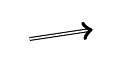
\begin{tikzpicture}\draw[->,double] (0,0)--(0.8,0.12);\end{tikzpicture}}}

\uline{Scholium} By the bijections (34) (38), we transport onto
$\unsure{g}_{\rho,\sigma},\ S_0g_{\rho,\sigma}$ the natural group structures
of $\unsure{\widetilde{\Gamma}_{\rho,\sigma}},\
\unsure{\Gamma^{b_0}_{\rho,\sigma}}$.
Making this group structure explicit we find in particular for $Sg_{\rho,\sigma}$
\[
\tag{\unsure{39|37}}
\left\{\begin{gathered}
(\alpha',\beta')(\alpha,\beta)=\alpha''\beta'',\quad
\text{with }\alpha''=u'(\alpha)\alpha',\quad\beta''=u'(\beta)\beta'.\\
u'=u_{\unsure{\zeta|\xi}',\eta'}:\
\diagram{\begin{tikzcd}[column sep=large]
\unsure{\mathcal{C}}\arrow[r] & \unsure{\mathcal{C}}
\end{tikzcd}},\quad\text{defined by }
\left\{\begin{aligned}
u(\rho)&=\unsure{\zeta|\xi}\rho=\operatorname{int}(\alpha)\rho\\
u(\sigma)&=\eta\sigma=\operatorname{int}(\beta)\sigma
\end{aligned}\right.
\end{gathered}\right.
\]
(with $\unsure{\zeta|\xi}=\alpha\rho(\alpha)^{-1},\ \eta=\beta\sigma(\beta)^{-1}$).

In $\unsure{S_0\Gamma^{b_0}_{\rho,\sigma}}$ we have a subgroup isomorphic to $L_0$, i.e.
\margin{\inserted{
\[
\tag{39}
\diagram{\begin{tikzcd}[column sep=large,row sep=small]
L_0\arrow[r] & \unsure{S\Gamma'_{\rho,\sigma}}\\
\unsure{\ell}\arrow[r,mapsto] & (\ell,1,1)
\end{tikzcd}}
\]
and we have exact sequence
\[
\tag{40}
\diagram{\begin{tikzcd}[column sep=small]
1\arrow[r] & L_0\arrow[r] & \unsure{S\Gamma'_{\rho,\sigma}}\arrow[r]
 & \unsure{\Gamma}_{\rho,\sigma}\arrow[r] & 1
\end{tikzcd}}
\]
}}

\deleted{
$\bullet$ \unsure{Let us now put}
\[
\tag{39}
\begin{gathered}
M_{\rho,\sigma}\subset\operatorname{Aut}(\unsure{\mathcal{C}})\\
\Vert\;\mathrm{dfn}\\
\left\{u\ \middle|\
\begin{array}{l}
\text{\unsure{a)|1°)} }u\ \deleted{\unsure{which}}\ \text{fixes the conjugacy classes of }\rho,\sigma\text{ in }\unsure{\mathcal{C}},\\
\quad\text{i.e. }\exists\alpha_0,\beta_0\in\unsure{\mathcal{C}}\ \deleted{\unsure{\text{such that}}}\ \text{with }\
u(\rho)=\operatorname{int}(\alpha_0)\rho,\quad u(\sigma)=\operatorname{int}(\beta_0)\sigma,\\
\text{\unsure{b)|2°)} }u\ \text{fixes the conjugacy class of }L_0,\\
\quad\text{i.e. }\exists f\in\unsure{\mathcal{C}}\ \text{such that }u(L_0)=\operatorname{int}(f^{-1}).L_0,\\
\quad\text{i.e. }fu\in\operatorname{Norm}_{\operatorname{Aut}(\unsure{\mathcal{C}})}(L_0)
\end{array}\right\}
\end{gathered}
\]
hence by definition of
\[
\tag{41}
\unsure{\mathcal{T}|\Gamma}_{\rho,\sigma}\overset{\mathrm{dfn}}{=}
Z_\rho\mathbin{\times}_{\Gamma_{\rho,\sigma}}Z_\sigma
\]
hence
\[
\tag{42}
\diagram{\begin{tikzcd}[column sep=small]
1\arrow[r] & SZ_\rho\times SZ_\sigma\arrow[r]
 & \unsure{\mathcal{T}|\Gamma}_{\rho,\sigma}\arrow[r,"\unsure{\delta_{\mathcal{T}}}"]
 & \Gamma_{\rho,\sigma}\arrow[r] & 1
\end{tikzcd}}
\]
}
\mspage{509}
